\subsection{График числовой последовательности}
График заданной числовой последовательности имеет следующий вид:

\begin{figure}[h]
	\centering
	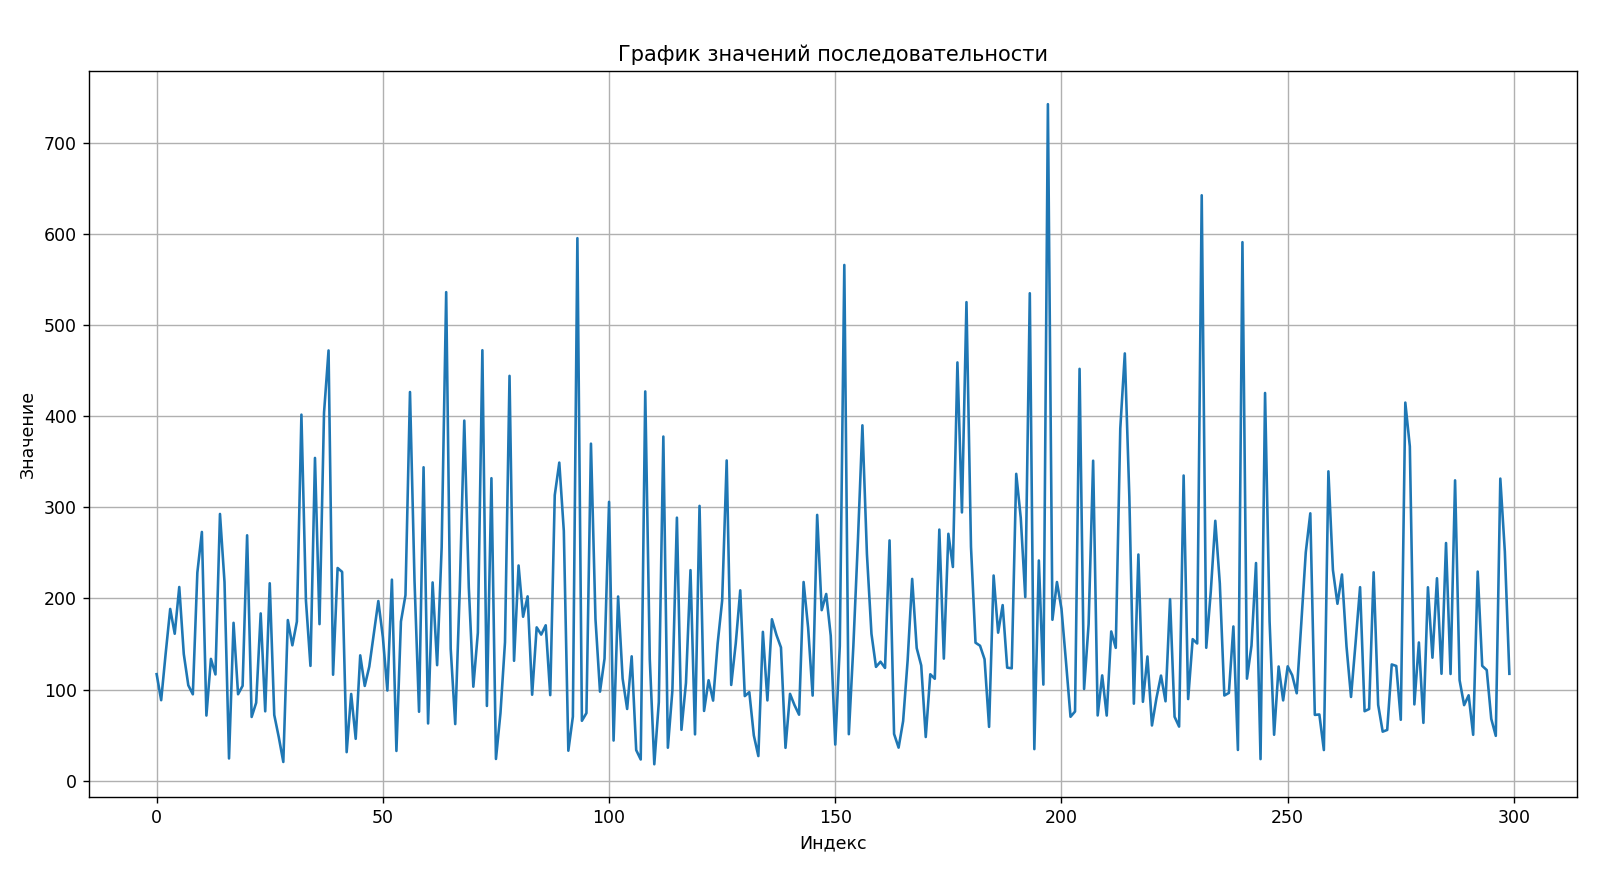
\includegraphics[width=1\textwidth]{../data/sequence.png}
	\caption{график числовой последовательности}
\end{figure}

\subsection{Анализ числовой последовательности}

Построив график числовой последовательности (Рис. 1), можно провести её анализ и определить характер распределения значений:

\begin{itemize}
	\item \textbf{Тренд (возрастающая/убывающая последовательность)}: График не демонстрирует явной тенденции роста или падения. Значения колеблются в случайном порядке, не показывая направленного изменения в какую-либо сторону. Следовательно, последовательность \textbf{не является ни возрастающей, ни убывающей}.

	\item \textbf{Периодичность}: На графике отсутствуют чёткие повторяющиеся паттерны. Это позволяет заключить, что последовательность \textbf{не является периодичной}.

	\item \textbf{Случайный характер}: Видимые колебания значений на графике происходят без какой-либо закономерности. Это указывает на \textbf{случайный характер} последовательности.
\end{itemize}

\subsection{Выводы}

Таким образом, по результатам анализа можно сделать вывод, что исследуемая числовая последовательность является \textbf{хаотичной} и не демонстрирует признаков \textbf{ни периодичности}, \textbf{ни направленного} изменения.
